\documentclass[a4paper, 12pt]{article}
\usepackage[utf8x]{inputenc}
\usepackage[english, russian]{babel}
\usepackage[left=25mm, top=25mm, right=25mm, bottom=25mm]{geometry}
\usepackage{cmap}
\usepackage{indentfirst}
\usepackage{tikz}
\usepackage{float}
\usepackage{amsmath, amsfonts, amssymb}
\usepackage{graphicx}
\usepackage{hyperref}
\usepackage{listings}
\usepackage{caption}
\usepackage{subcaption}
\usepackage{xcolor}
\usepackage{etoolbox}
\usepackage{titlesec}
\usepackage{array}
\pagestyle{plain}
\patchcmd{\tableofcontents}{\contentsname}{\centering\contentsname}{}{}
\titleformat{\section}[block]{\normalfont\large\bfseries\centering}{}{0pt}{}
\titleformat{\subsection}[block]{\normalfont\normalsize\bfseries\centering}{}{0pt}{}
\titleformat{\subsubsection}[block]{\normalfont\small\bfseries\centering}{}{0pt}{}
\allowdisplaybreaks
\graphicspath{{src/images/}}
\usetikzlibrary{patterns}
\definecolor{LightGray}{gray}{0.95}
\definecolor{LightGray2}{gray}{0.7}
\hypersetup{
    colorlinks=true,
    linkcolor=blue,
    filecolor=magenta,
    urlcolor=cyan,
    pdftitle={contents setup},
    pdfpagemode=FullScreen,
}


\begin{document}
    \begin{titlepage}

        \begin{center}
        Федеральное государственное автономное образовательное учреждение высшего образования
        «Национальный Исследовательский Университет ИТМО»
        \vfill
        
        
\includegraphics[width=0.3\textwidth]{itmo.png} % requires /src/images/itmo.png

        {\large\bf ЛАБОРАТОРНАЯ РАБОТА №6}\\
        {\large\bf ПРЕДМЕТ «ЭЛЕКТРОННЫЕ УСТРОЙСТВА СИСТЕМ УПРАВЛЕНИЯ»}\\
        {\large\bf ТЕМА «ИСТОЧНИКИ ТОКА»}
        \vfill

        \begin{flushright}
            \begin{minipage}{.45\textwidth}
            {
                \hbox{Преподаватель:}
                \hbox{Жданов В. А.}
                \hbox{}
                \hbox{Выполнил:}
                \hbox{Румянцев А. А.}
                \hbox{}
                \hbox{Факультет: СУиР}
                \hbox{Группа: R3341}
                \hbox{Поток: ЭлУСУ R22 бак 1.2}
            }
            \end{minipage}
        \end{flushright}
        \vfill
  
        Санкт-Петербург\\
        2025
        \end{center}
    \end{titlepage}
    
    \tableofcontents

    \newpage
    \section{Цель работы}
    Цель работы -- исследование работы источников тока.


    \section{Исследование токового зеркала с компенсацией теплового дрейфа}
    \subsection{Расчет схемы}
    Рассчитаем схему токового зеркала с компенсацией теплового дрейфа.
    Дан ток нагрузки $$I_\text{Н}=250\text{ мА}$$
    и следующие формулы
    $$
    I_{k1}\approx\dfrac{E_\text{П}-0.7}{R_1+R_\text{э1}},\ I_\text{Н}\approx\dfrac{R_\text{э1}\left( E_\text{П}-0.7 \right)}{R_1R_\text{э2}+R_\text{э1}R_\text{э2}};
    $$
    Зададим напряжение питания $$E_\text{П}=12\text{ В}$$
    Кремниевые транзисторы обычно имеют напряжение между базой и и эмиттером
    $$
    U_\text{БЭ}=0.7\text{ В}
    $$
    Так как токовое зеркало <<копирует>> ток через первый транзистор, то ток через
    нагрузку должен быть равен току на первом транзисторе
    $$
    I_{k1}\approx I_\text{Н}=250\text{ мА}
    $$
    Найдем сумму сопротивлений $R_1+R_\text{э1}$ через формулу для $I_{k1}$
    $$
    250\cdot10^{-3}=\dfrac{12-0.7}{R_1+R_\text{э1}}\Rightarrow R_1+R_\text{э1}=\dfrac{11.3}{0.25}=45.2\text{ Ом}
    $$
    Для уменьшения потерь мощности выберем первый эмиттерный резистор с небольшим номиналом в 10 Ом. Рассчитаем $R_1$
    $$
    R_\text{э1}=10\text{ Ом}\Rightarrow R_1=45.2-10=35.2\text{ Ом}
    $$
    Ближайший стандартный номинал $R_1\approx35$ Ом. Рассчитаем сопротивление второго эмиттерного резистора $R_\text{э2}$ через формулу для $I_\text{Н}$
    $$
    250\cdot10^{-3}=\dfrac{10\left( 12-0.7 \right)}{35R_\text{э2}+10R_\text{э2}}\Rightarrow R_\text{э2}=\dfrac{113}{0.25\cdot45}\approx10.04\text{ Ом}
    $$
    Возьмем ближайший стандартный номинал $R_\text{э2}\approx10$ Ом. Выберем в качестве T1 T2 транзисторов 2N2222 из библиотеки LTspice.
    Напряжение между коллектором и эмиттером этого транзистора, когда он находится в режиме насыщения, составляет
    $$
    U_\text{КЭ (нас)}\approx0.2\text{ В}
    $$
    Тогда, определим сопротивление нагрузочного резистора по формуле
    $$
    R_\text{Н}=\dfrac{E_\text{П}-U_\text{КЭ (нас)}}{I_\text{Н}}=\dfrac{12-0.2}{250\cdot10^{-3}}=\dfrac{11.8}{0.25}=47.2\text{ Ом}
    $$
    Ближайший стандартный номинал $R_\text{Н}\approx47$ Ом.


    \subsection{Схема токового зеркала с компенсацией теплового дрейфа}
    Построим в LTspice одноименную схему
    \begin{figure}[H]
        \centering
        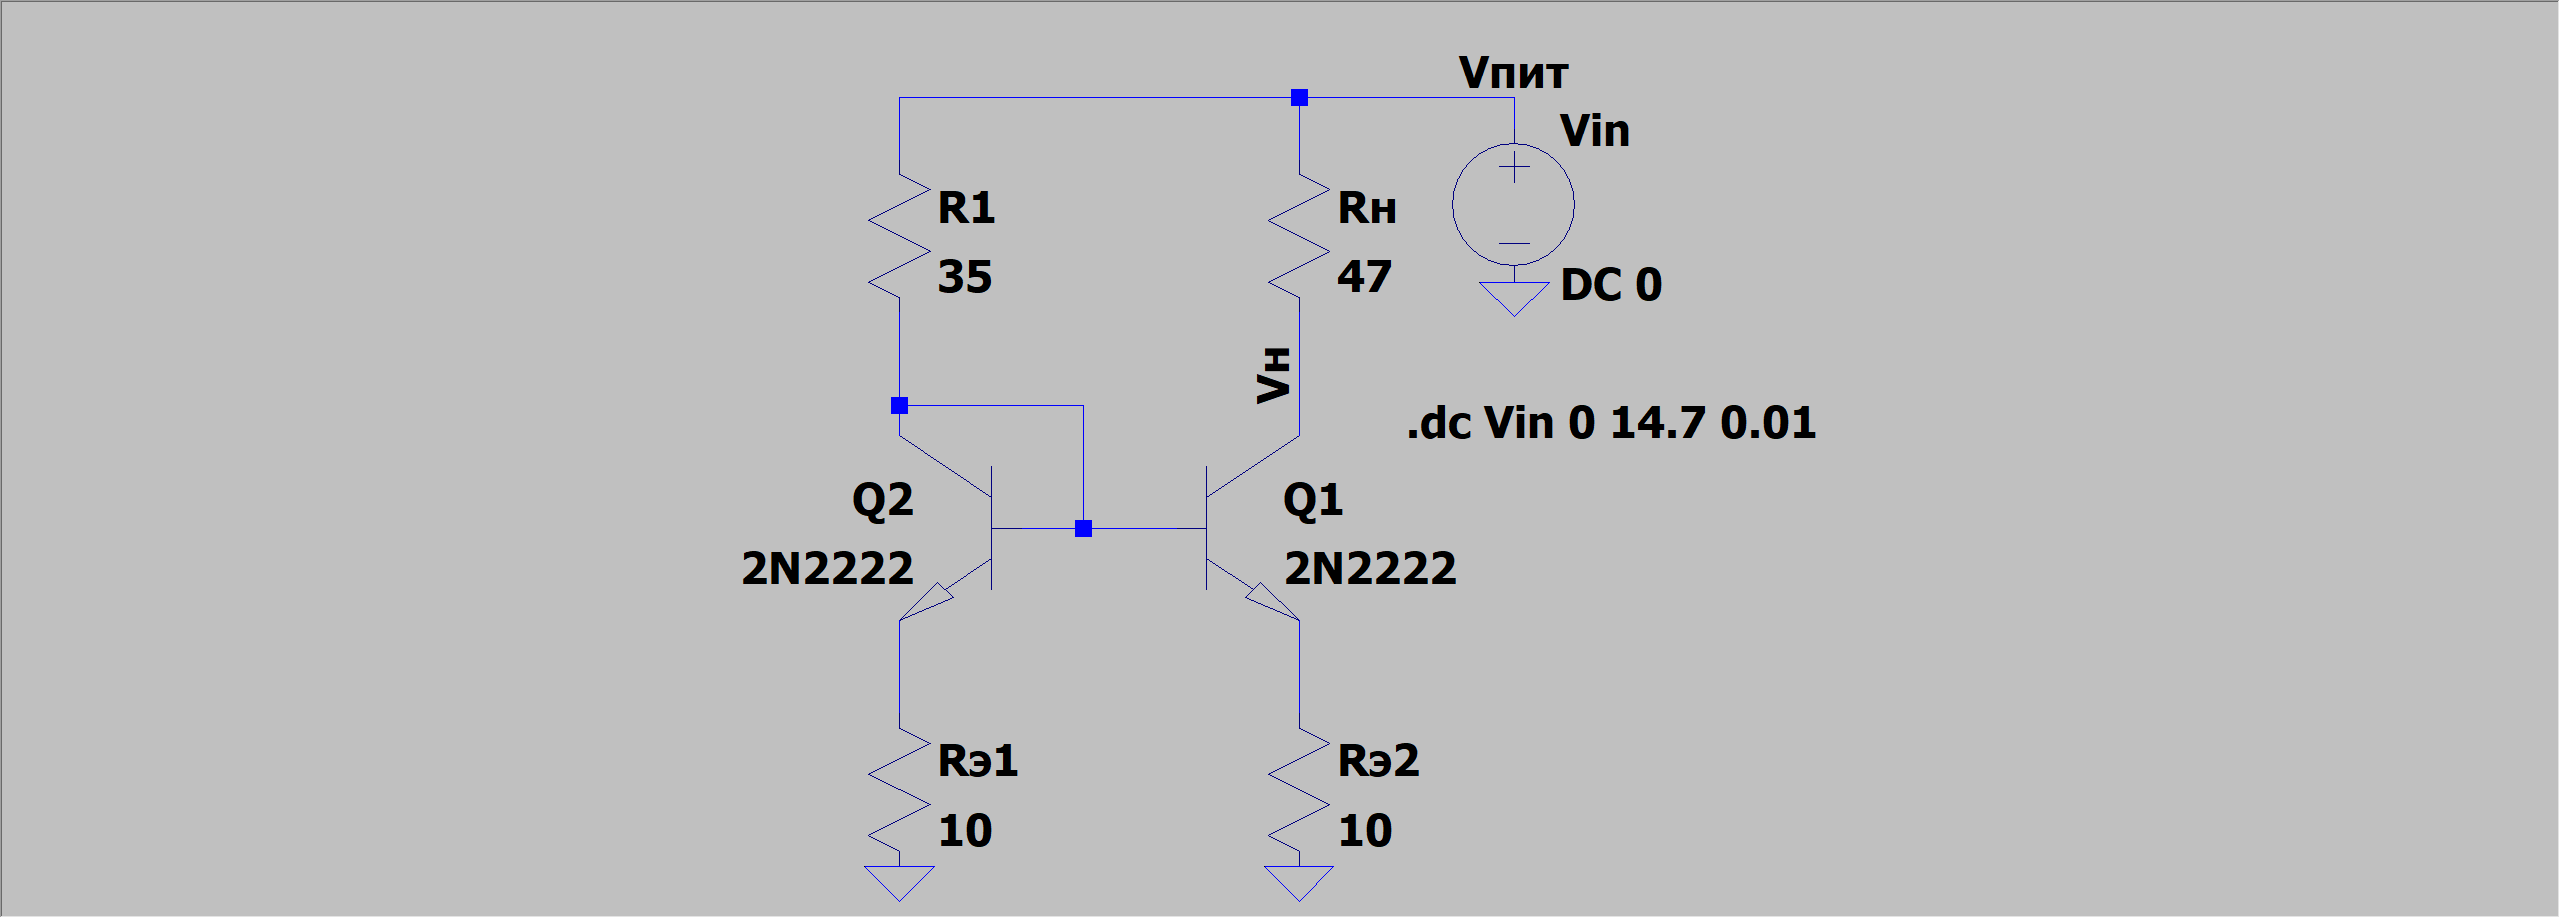
\includegraphics[scale=0.22]{scheme1.png}
        \captionsetup{skip=0pt}
        \caption{Схема токового зеркала с компенсацией теплового дрейфа}
        \label{fig:scheme1}
    \end{figure}


    \subsection{Зависимость тока через нагрузку от напряжения на нагрузке}
    Построим график зависимости тока через нагрузку от напряжения на нагрузке.
    Зададим в источник питания DC 0, поставим на схему .dc Vin 0 14.7 0.01.
    С помощью net обозначим Vн
    \begin{figure}[H]
        \centering
        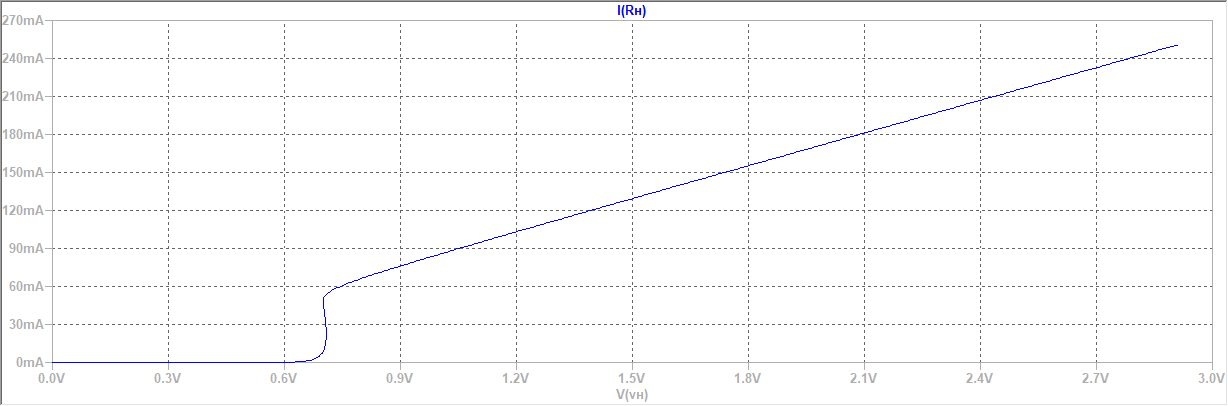
\includegraphics[scale=0.46]{1task_Iн(Vн).png}
        \captionsetup{skip=0pt}
        \caption{Зависимость $I_\text{Н}$ от $U_\text{Н}$}
        \label{fig:1task_InVn}
    \end{figure}
    \noindent Биполярный транзистор начинает проводить только когда между базой
    и эмиттером набирается напряжение примерно в $0.6$--$0.7$ В. До этого момента
    оба транзистора в зеркале закрыты -- ток не течет.


    \subsection{Зависимость тока через нагрузку и тока на токозадающем устройстве от напряжения питания}
    Построим график зависимости тока через нагрузку и тока на токозадающем устройстве от напряжения питания.
    С помощью net обозначим Vпит. Синяя траектория -- зависимость тока через нагрузку от напряжения питания,
    красный -- зависимость тока на токозадающем устройстве от напряжения питания
    \begin{figure}[H]
        \centering
        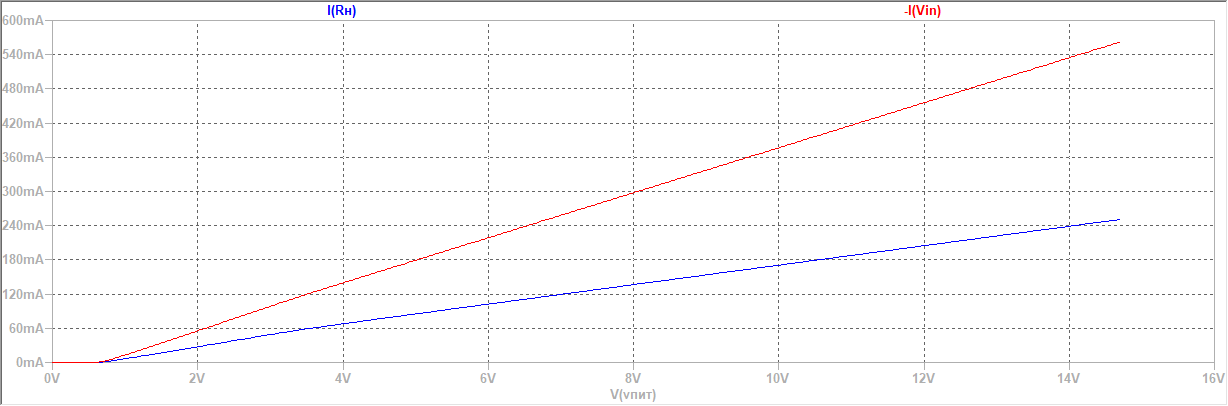
\includegraphics[scale=0.46]{1task_Iн(Vпит)_Iпит(Vпит).png}
        \captionsetup{skip=0pt}
        \caption{Зависимости $I_\text{Н}\left( U_\text{пит} \right),\ I_\text{пит}\left( U_\text{пит} \right)$}
        \label{fig:1task_InVl_IlVl}
    \end{figure}
    \noindent Токи равны нулю до напряжения в 0.7 В.
    Ток питания больше, так как он включает в себя ток через нагрузку,
    ток через токозадающее плечо Q1 и базовые токи обоих транзисторов.


    \subsection{Ток через нагрузку при различных сопротивлениях нагрузки}
    Построим графики зависимости тока от напряжения питания при различных сопротивлениях нагрузки.
    Проверим $R_\text{Н}=10,10^2,10^3,10^4$ Ом. Красный график -- подаваемое напряжение питания,
    синий -- ток нагрузки
    \begin{figure}[H]
        \centering
        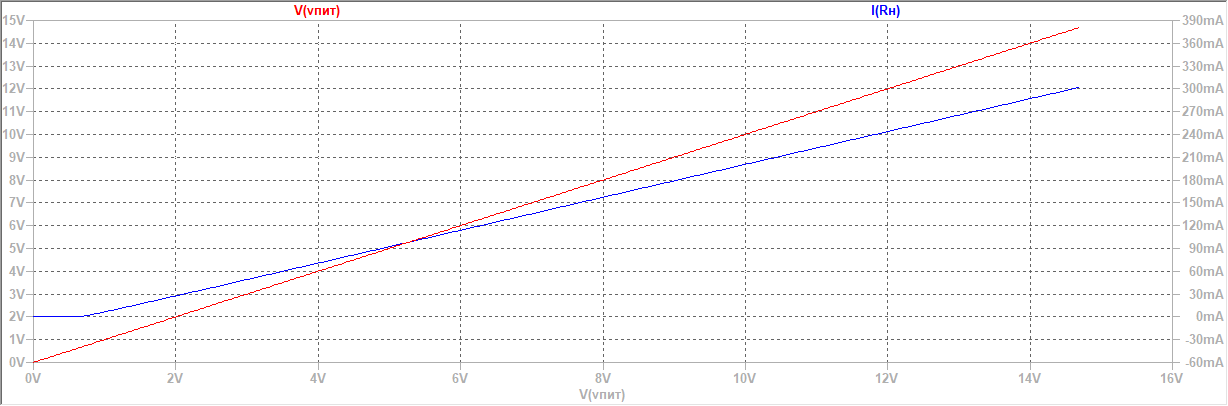
\includegraphics[scale=0.46]{1task_Iн(Vпит)_Rн10.png}
        \captionsetup{skip=0pt}
        \caption{$I_\text{Н}\left( U_\text{пит} \right)$ при $R_\text{Н}=10$ Ом}
        \label{fig:1task_InVlR10}
    \end{figure}
    \begin{figure}[H]
        \centering
        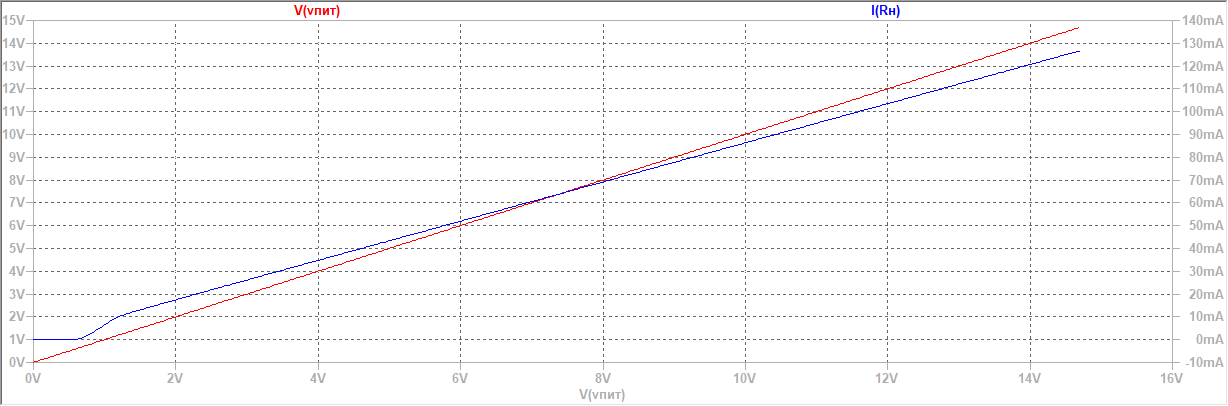
\includegraphics[scale=0.46]{1task_Iн(Vпит)_Rн100.png}
        \captionsetup{skip=0pt}
        \caption{$I_\text{Н}\left( U_\text{пит} \right)$ при $R_\text{Н}=100$ Ом}
        \label{fig:1task_InVlR100}
    \end{figure}
    \begin{figure}[H]
        \centering
        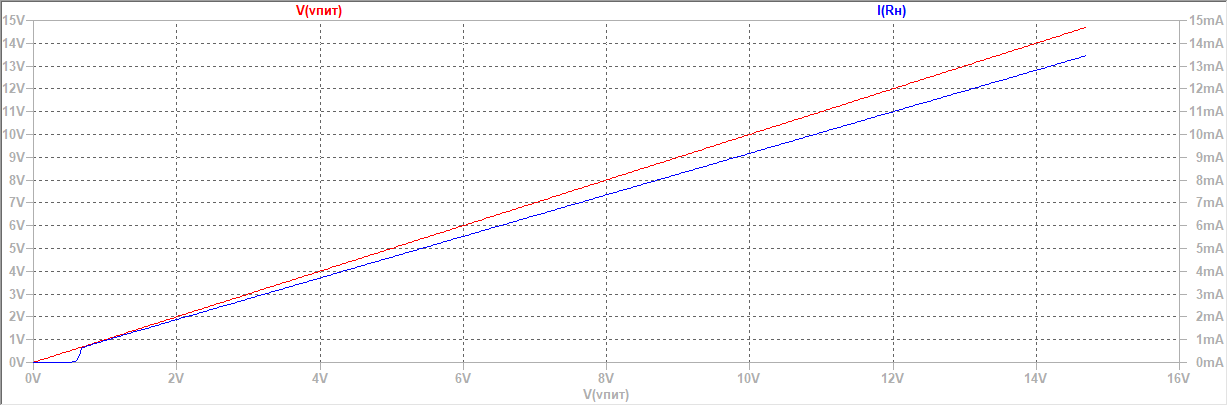
\includegraphics[scale=0.46]{1task_Iн(Vпит)_Rн1000.png}
        \captionsetup{skip=0pt}
        \caption{$I_\text{Н}\left( U_\text{пит} \right)$ при $R_\text{Н}=1000$ Ом}
        \label{fig:1task_InVlR1000}
    \end{figure}
    \begin{figure}[H]
        \centering
        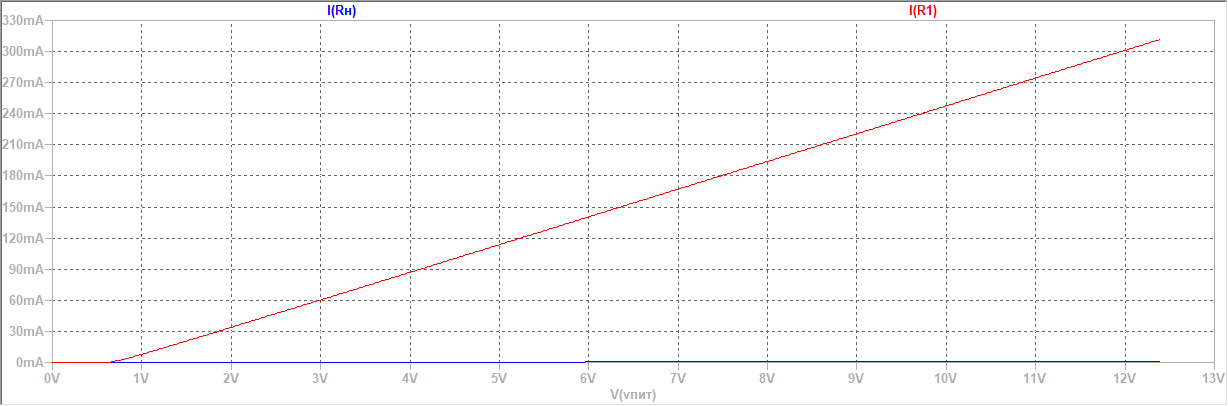
\includegraphics[scale=0.46]{1task_Iн(Vпит)_Rн10000.png}
        \captionsetup{skip=0pt}
        \caption{$I_\text{Н}\left( U_\text{пит} \right)$ при $R_\text{Н}=10000$ Ом}
        \label{fig:1task_InVlR10000}
    \end{figure}
    \noindent При увеличении сопротивления нагрузки ток нагрузки уменьшается -- токовое зеркало не может создать нужный ток,
    не хватает напряжения питания.


    \section{Исследование токового зеркала Уилсона}
    \subsection{Расчет схемы}
    Рассчитаем схему токового зеркала Уилсона. Дан ток нагрузки
    $$
    I_\text{Н}=250\text{ мА}
    $$
    и следующие формулы
    $$
    I_{k1}\approx\dfrac{E_\text{П}-1.4}{R_1+R_\text{э1}},\ I_\text{Н}\approx\dfrac{R_\text{э1}\left( E_\text{П}-0.7 \right)}{R_1R_\text{э2}+R_\text{э1}R_\text{э2}};
    $$
    Зададим напряжение питания $$E_\text{П}=12\text{ В}$$
    Эмиттерное напряжение для кремниевого транзистора
    $$
    U_\text{БЭ}=0.7\text{ В}
    $$
    Ток через нагрузку $I_\text{Н}$ должен быть равен $I_{k1}$, так как токовое зеркало копирует ток через первый транзистор Q1
    $$
    I_{k1}\approx I_\text{Н}=250\text{ мА}
    $$
    Найдем сумму $R_1+R_\text{э1}$ из формулы для $I_{k1}$
    $$
    250\cdot10^{-3}=\dfrac{12-1.4}{R_1+R_\text{э1}}\Rightarrow R_1+R_\text{э1}=\dfrac{10.6}{0.25}=42.4\text{ Ом}
    $$
    Пусть $R_\text{э1}=10$ Ом, тогда
    $$
    R_1=42.4-10=32.4
    $$
    Возьмем ближайший стандартный номинал $R_1\approx33$ Ом. Используя формулу для $I_\text{Н}$,
    определим $R_\text{э2}$
    $$
    250\cdot10^{-3}=\dfrac{10\left( 12-0.7 \right)}{33R_\text{э2}+10R_\text{э2}}\Rightarrow R_\text{э2}=\dfrac{113}{0.25\cdot43}\approx10.51\text{ Ом}
    $$
    Возьмем ближайший стандартный номинал $R_\text{э2}\approx10$ Ом. В качестве транзисторов T1 T2 T3 выберем 2N2222
    из библиотеки LTspice. Аналогично имеем
    $$
    U_\text{КЭ (нас)}\approx0.2\text{ В}
    $$
    Тогда, сопротивление на нагрузке
    $$
    R_\text{Н}=\dfrac{E_\text{П}-U_\text{КЭ (нас)}}{I_\text{Н}}=\dfrac{12-0.2}{250\cdot10^{-3}}=47.2\text{ Ом}
    $$
    Ближайший стандартный номинал $R_\text{Н}\approx47$ Ом.


    \subsection{Схема токового зеркала Уилсона}
    Построим в LTspice одноименную схему
    \begin{figure}[H]
        \centering
        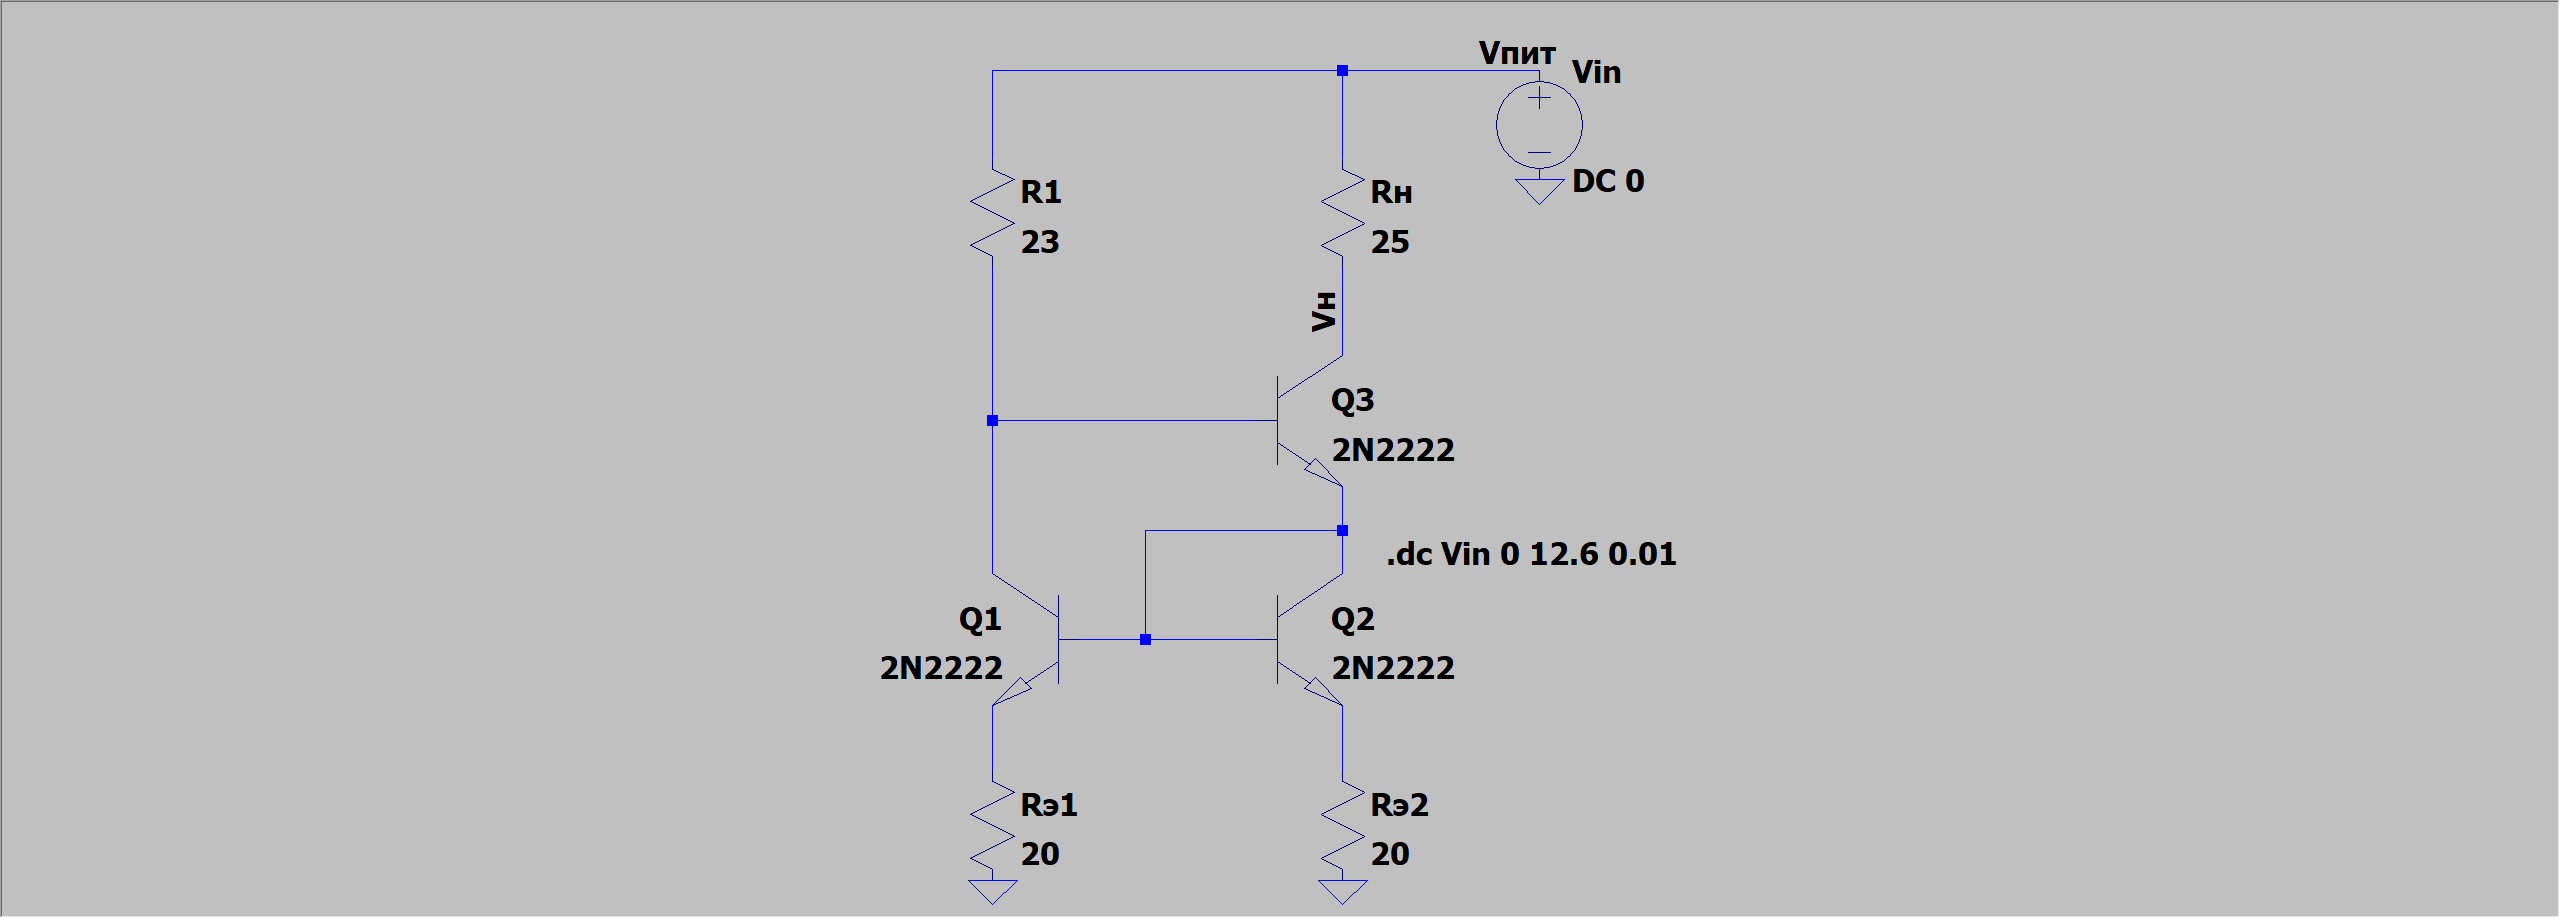
\includegraphics[scale=0.22]{scheme2.png}
        \captionsetup{skip=0pt}
        \caption{Схема токового зеркала Уилсона}
        \label{fig:scheme2}
    \end{figure}


    \subsection{Зависимость тока через нагрузку от напряжения на нагрузке}
    Построим график зависимости тока через нагрузку от напряжения на нагрузке.
    Зададим в источник питания DC 0, поставим на схему .dc Vin 0 15.7 0.01.
    С помощью net обозначим Vн
    \begin{figure}[H]
        \centering
        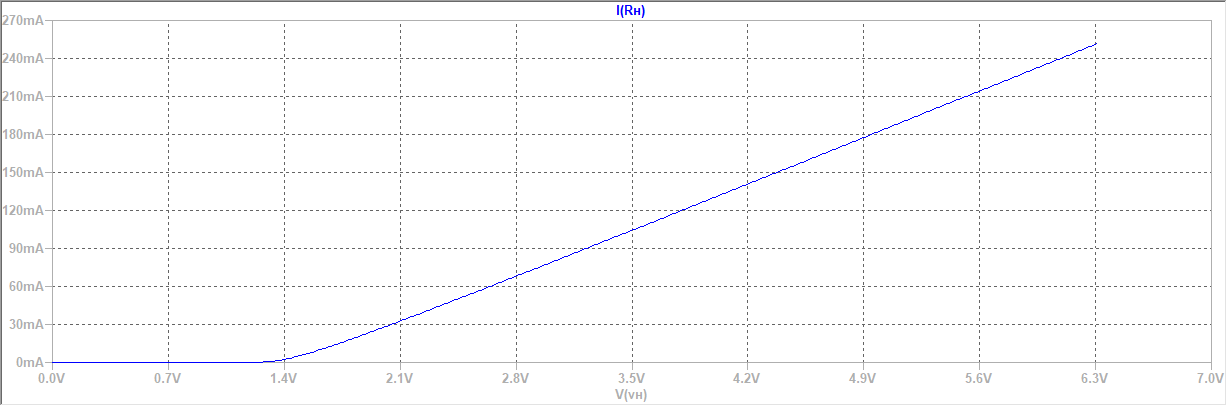
\includegraphics[scale=0.46]{2task_Iн(Vн).png}
        \captionsetup{skip=0pt}
        \caption{Зависимость $I_\text{Н}$ от $U_\text{Н}$}
        \label{fig:2task_InVn}
    \end{figure}
    \noindent Имеем два последовательных перехода база-эмиттер, что дает в сумме падение напряжения на 1.4 В.
    На графике видим, что транзисторы открываются в районе 1.4 В, до этого момента ток нулевой.


    \subsection{Зависимость тока через нагрузку и тока на токозадающем устройстве от напряжения питания}
    Построим график зависимости тока через нагрузку и тока на токозадающем устройстве от напряжения питания.
    С помощью net обозначим Vпит. Синяя траектория -- зависимость тока через нагрузку от напряжения питания,
    красный -- зависимость тока на токозадающем устройстве от напряжения питания
    \begin{figure}[H]
        \centering
        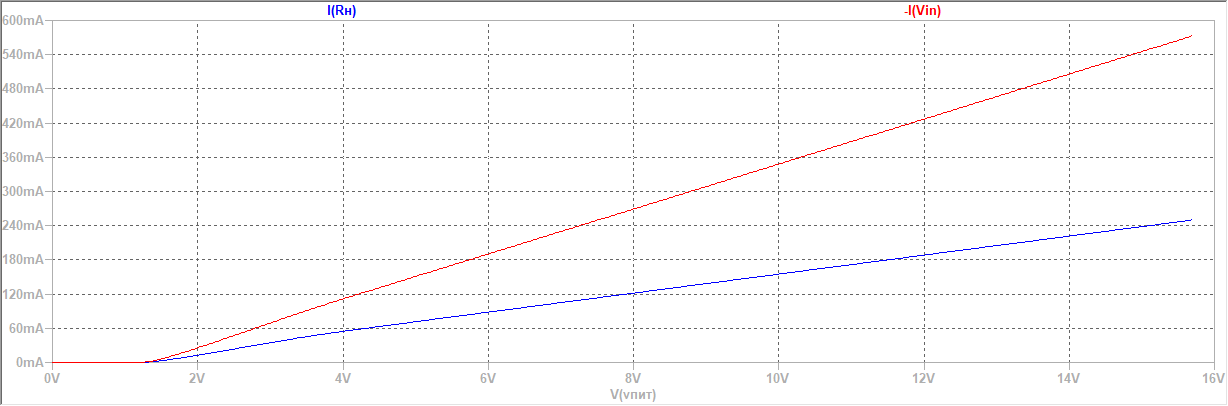
\includegraphics[scale=0.46]{2task_Iн(Vпит)_Iпит(Vпит).png}
        \captionsetup{skip=0pt}
        \caption{Зависимости $I_\text{Н}\left( U_\text{пит} \right),\ I_\text{пит}\left( U_\text{пит} \right)$}
        \label{fig:2task_InVl_IlVl}
    \end{figure}
    \noindent До напряжения в 1.4 В транзисторы закрыты, ток нулевой. После они входят в активный режим,
    ток растет линейно. Максимумы $I_\text{Н}\approx251$ мА, $I_\text{пит}\approx574$ мА. Ток
    на токозадающем устройстве больше, так как включает в себя оба токовых плеча и базовые токи транзисторов.
    Для достижения $I_\text{Н}=250$ мА потребовалось подать напряжение на 1 В больше, чем в случае
    с токовым зеркалом с компенсацией теплового дрейфа.


    \subsection{Ток через нагрузку при различных сопротивлениях нагрузки}
    Построим графики зависимости тока от напряжения питания при различных сопротивлениях нагрузки.
    Проверим $R_\text{Н}=10,10^2,10^3,10^4$ Ом. Красный график -- подаваемое напряжение питания,
    синий -- ток нагрузки
    \begin{figure}[H]
        \centering
        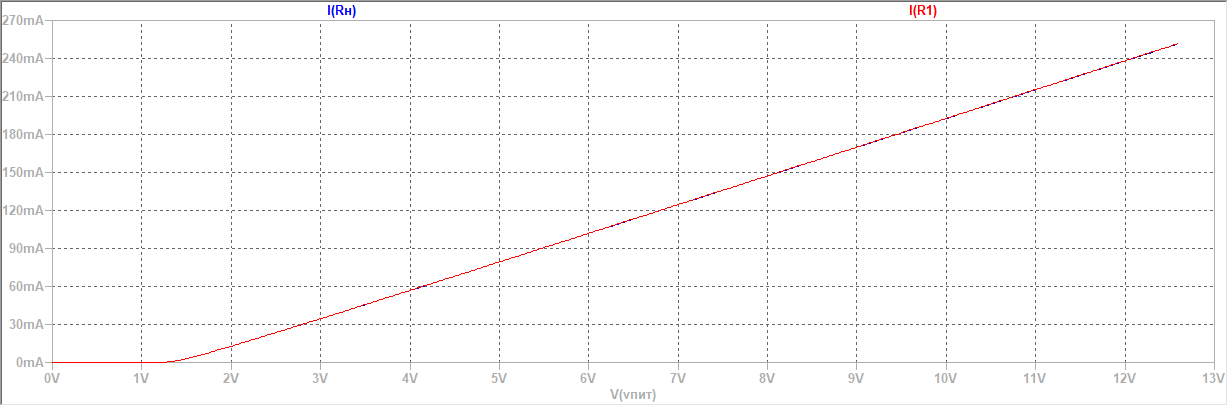
\includegraphics[scale=0.46]{2task_Iн(Vпит)_Rн10.png}
        \captionsetup{skip=0pt}
        \caption{$I_\text{Н}\left( U_\text{пит} \right)$ при $R_\text{Н}=10$ Ом}
        \label{fig:2task_InVlR10}
    \end{figure}
    \begin{figure}[H]
        \centering
        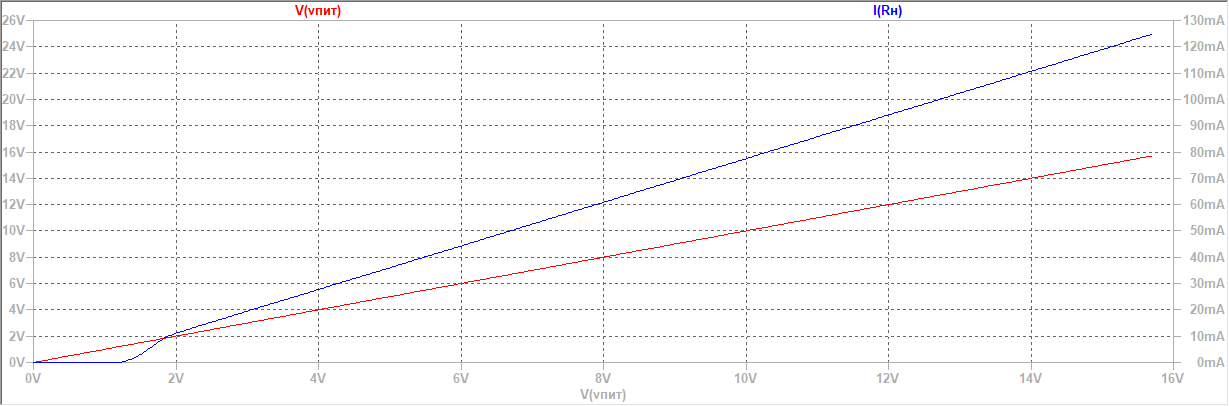
\includegraphics[scale=0.46]{2task_Iн(Vпит)_Rн100.png}
        \captionsetup{skip=0pt}
        \caption{$I_\text{Н}\left( U_\text{пит} \right)$ при $R_\text{Н}=100$ Ом}
        \label{fig:2task_InVlR100}
    \end{figure}
    \begin{figure}[H]
        \centering
        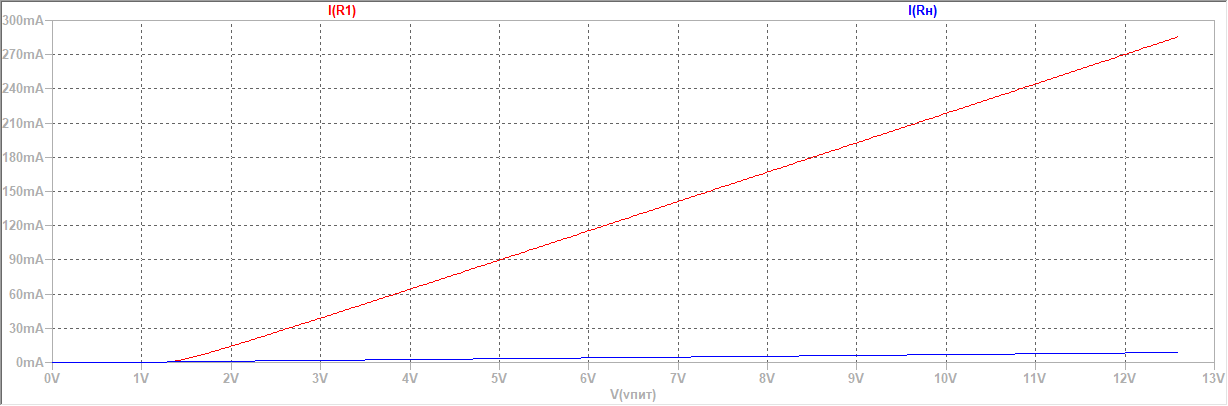
\includegraphics[scale=0.46]{2task_Iн(Vпит)_Rн1000.png}
        \captionsetup{skip=0pt}
        \caption{$I_\text{Н}\left( U_\text{пит} \right)$ при $R_\text{Н}=1000$ Ом}
        \label{fig:2task_InVlR1000}
    \end{figure}
    \begin{figure}[H]
        \centering
        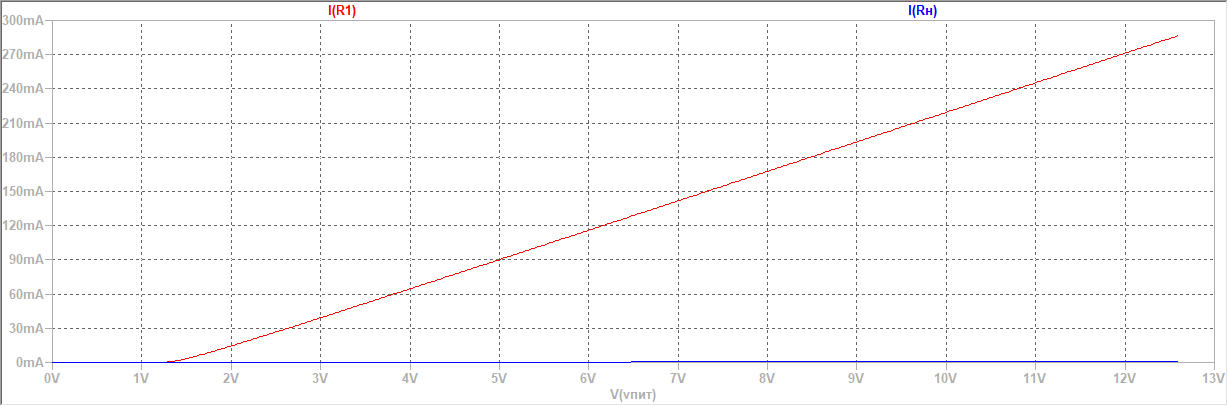
\includegraphics[scale=0.46]{2task_Iн(Vпит)_Rн10000.png}
        \captionsetup{skip=0pt}
        \caption{$I_\text{Н}\left( U_\text{пит} \right)$ при $R_\text{Н}=10000$ Ом}
        \label{fig:2task_InVlR10000}
    \end{figure}
    \noindent При увеличении сопротивления нагрузки ток нагрузки уменьшается.
    В сравнении с токовым зеркалом с компенсацией теплового дрейфа падение тока более заметно.
    Транзистор быстрее уходит в насыщение и не может поддерживать заданный ток -- не хватает напряжения.
\end{document} 